\section{Signal Extraction}

The presence of DM production will be observable as an excess of events with respect to the expectations for the 
SM backgrounds in a region at high missing transverse energy. Significant improvements in terms of sensitivity can be expected if 
several bins in $\ETm$ are considered simultaneously. 
A binned likelihood fit is performed in the range 250 \gev to 1000 \gev (or 200 \gev to 1000 \gev 
for the monojet category), where the binning is chosen to ensure each corresponding bin of the control regions  
is populated. The width of the highest $\ETm$ bin allows for ease of comparison to the previous CMS search~\cite{monojet1}. 

Data from three control regions, the dimuon and photon control regions, and the single-muon control region, are used to determine the contributions from \Zvvjets~and 
\Wlvjets~respectively. The events in the control regions are divided into the three  categories, using the same selection criteria as 
described in Section~\ref{sec:selection}. In the dimuon, single-muon and photon control regions, the dimuon pair, single-muon or the photon's 
momentum are removed and the \ETm ~is recalculated yielding a distribution of fake \ETm. The distribution of fake \ETm 
in data in the control regions is used to derive the expectation from the Z+jets and W+jets backgrounds in the signal region.

As the decay branching ratio of \Zmm~is approximately 6 times smaller than that to neutrinos, the resulting statistical 
uncertainty on the \Zvvjets~template becomes a dominant systematic uncertainty at large values of \ETm.
A complementary approach is to use events in data that have a high-$p_{T}$ 
photon recoiling against jets to further constrain the \Zvvjets~background template~\cite{CMS-PAS-SUS-08-002}. This is advantageous since the production cross-section 
of \phojets~is roughly 3 times that of the \Zvvjets~resulting in a smaller statistical uncertainty on the predicted background. 
 
The \ETm spectra of the V+jets backgrounds is determined through the use of a likelihood fit, simultaneously across all bins 
in the three control regions. 
The expected number of events $N_{i}$ in a given bin $i$ of fake \ETm, for a particular event category, is given by, 
$N^{Z_{\mu\mu}|\gamma }_{i}=  \dfrac{{\mu^{\Zvv}_{i}}}{R^{Z|\gamma}_{i}}$, 
for the dimuon and photon control regions and  $N^{W}_{i} =  \dfrac{{\mu^{\Wlv}_{i}}}{R^{W}_{i}}$,
for the single-muon control region. The parameters $\boldsymbol{\mu}^{\Zvv}$ and $\boldsymbol{\mu}^{\Wlv}$ are the free parameters 
of the likelihood representing the yields of $\Zvvjets$ and $\Wlvjets$ in each bin of the signal region. The likelihood function for a 
particular category, $c$, is given as,   

\begin{align*}
\mathcal{L}_{\textrm{c}}(\boldsymbol{\mu}^{\textrm{c},\Zvv},\boldsymbol{\mu}^{\textrm{c},\Wlv},\boldsymbol{\theta},\boldsymbol{\phi}) &=        
                \prod_{i} \mathrm{Poisson}\left(d^{\textrm{c},\gamma}_{i} |B^{\textrm{c},\gamma}_{i}(\boldsymbol{\phi}) +\frac{ \mu^{\textrm{c},\Zvv}_{i} }{R^{\textrm{c},\gamma}_{i}(\boldsymbol{\theta})}   \right) \\
       &~\times \prod_{i} \mathrm{Poisson}\left(d^{\textrm{c},Z}_{i}      |B^{\textrm{c},Z}_{i}(\boldsymbol{\phi})      +\frac{ \mu^{\textrm{c},\Zvv}_{i} }{R^{\textrm{c},Z}_{i}     (\boldsymbol{\theta})}       \right ) \\
       &~\times \prod_{i} \mathrm{Poisson}\left(d^{\textrm{c},W}_{i}      |B^{\textrm{c},W}_{i}(\boldsymbol{\phi})      +\frac{ \mu^{\textrm{c},\Wlv}_{i} }{R^{\textrm{c},W}_{i}     (\boldsymbol{\theta})}       \right), \numberthis\label{eqn:candclh}
\end{align*}

where $d^{c,\gamma/Z/W}_{i}$ are the observed number of events in each bin of the photon, dimuon and single-muon control regions.
The expected contributions from background processes in the dimuon, single-muon and photon control regions are denoted $B^{Z}$, $B^{W}$ and 
$B^{\gamma}$ in equation~\ref{eqn:candclh} respectively.

The transfer factors $R^{Z}_{i}$ account for the ratio of $BR(\Zvv)/BR(\Zmm)$ and 
the muon efficiency times acceptance in the dimuon control region, while 
$R^{\gamma}_{i}$ account for the ratio of differential cross-sections between the Z+jet 
and photon+jet processes and the efficiency times acceptance of the photon selection for 
the photon plus jet control region. The differential boson $p_{T}$ cross-sections of 
photon and Z production are first corrected using NLO k-factors derived by  
comparing their $p_{T}$ distributions in events generated at single parton level with Madgraph5\_aMC@NLO~\cite{amcatnlo}, and subsequently showered,  
to the distributions produced at leading order before deriving the transfer factors. 

Systematic uncertainties are modelled as constrained nuisance parameters, $\boldsymbol{\theta}$, which allow for variation of 
the transfer factors, $R^{\gamma/Z/W}$, in the fit and are treated as fully correlated between event categories.
These include theoretical uncertainties on the photon to Z differential cross-section ratio from renormalization and factorization scale uncertainties. 
Electroweak corrections to the ratio are not accounted for in the simulation. The full correction is also taken as an uncertainty on the ratio, 
which is of the order of 15\% when the boson (Z or $\gamma$) \pt is at the TeV scale~\cite{Kuhn:2005gv}. A conservative choice is made in assuming 
this uncertainty to be uncorrelated across bins of \ETm. Additionally, the uncertainty in the muon selection efficiency, photon selection efficiency, 
and photon purity are included and fully correlated across the event categories and control regions, where relevant. A systematic uncertainty of 10\% 
is included for the background normalization~\cite{tagkey2015250} and correlated between the single-muon and dimuon control regions. The results of a fit to the control regions are shown in Figure~\ref{fig:combined_fit_result}.
 
\begin{figure*}[hbtp]\begin{center}
 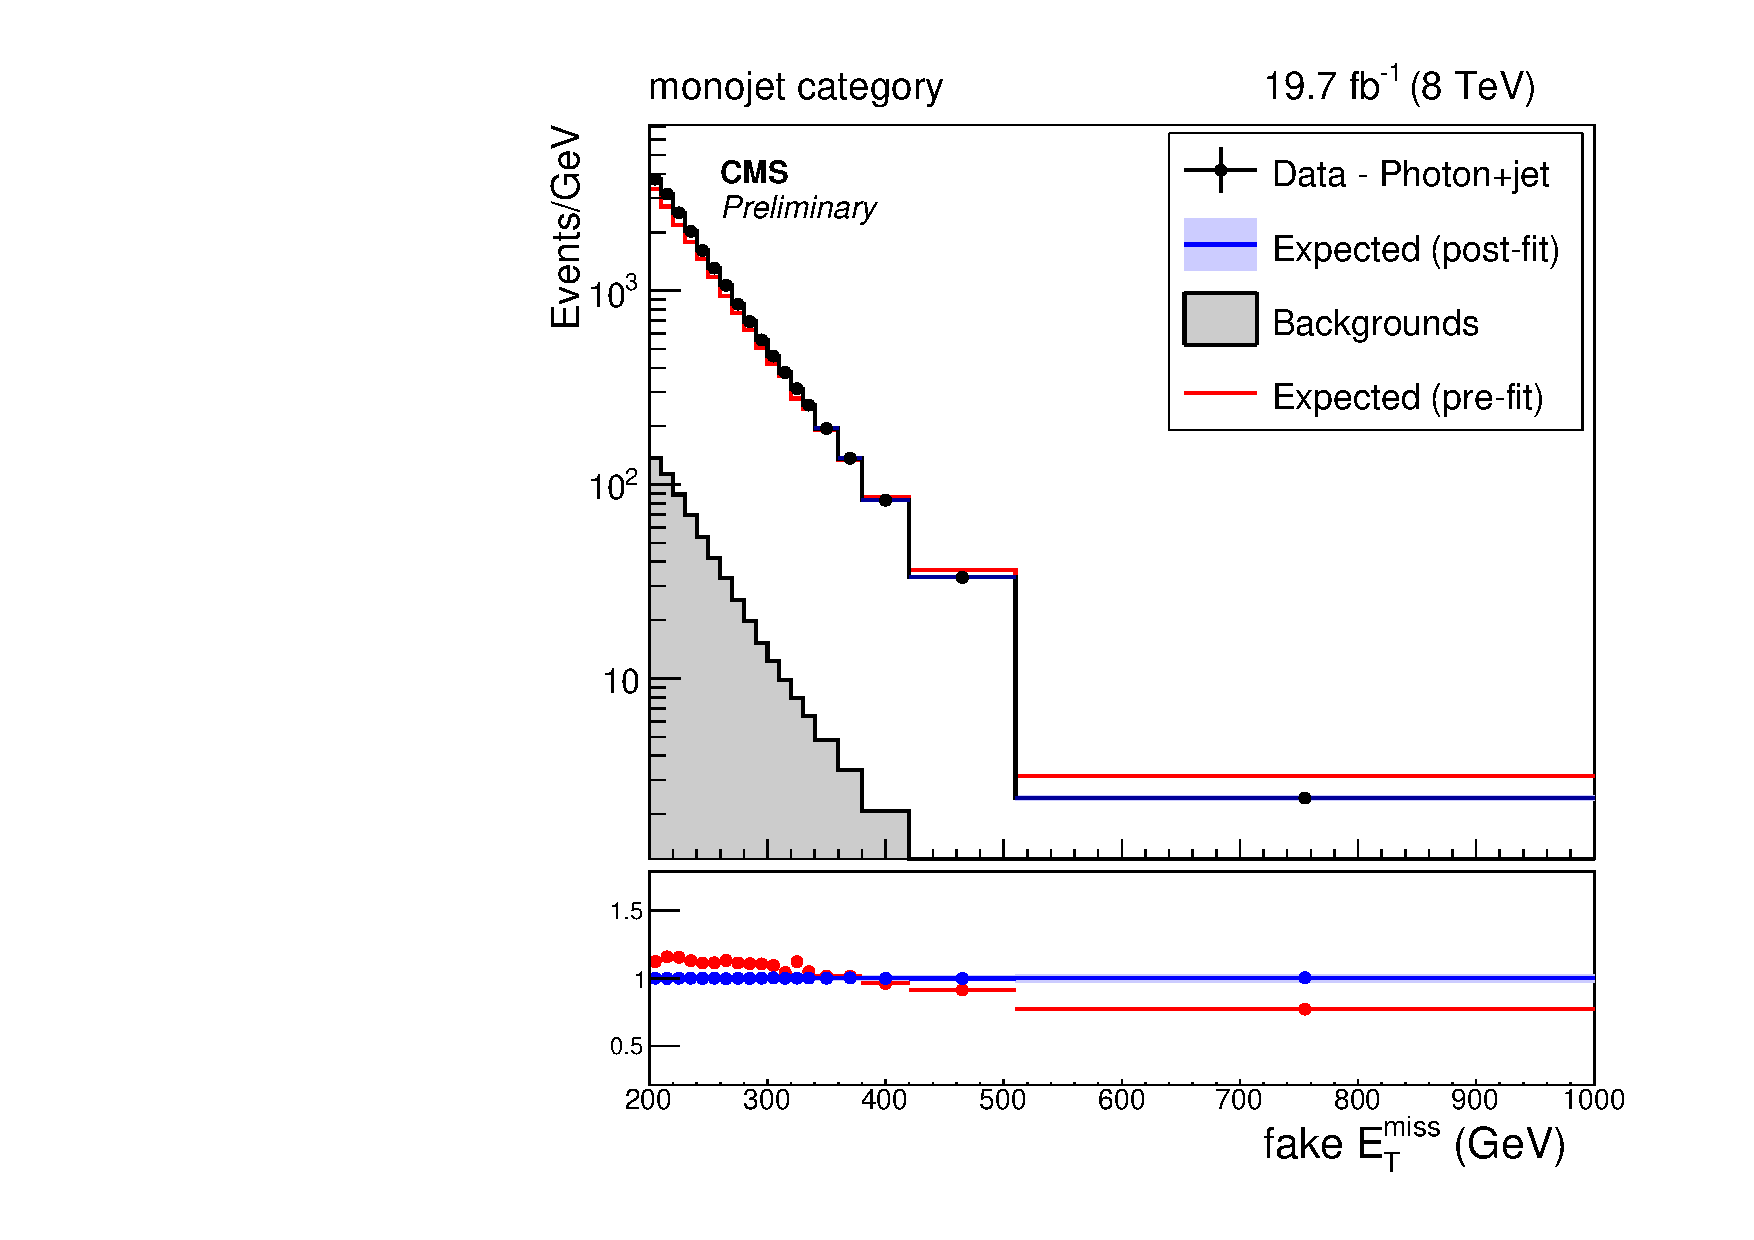
\includegraphics[width=0.32\textwidth]{figures/post_fit_photon_monojet.pdf}
 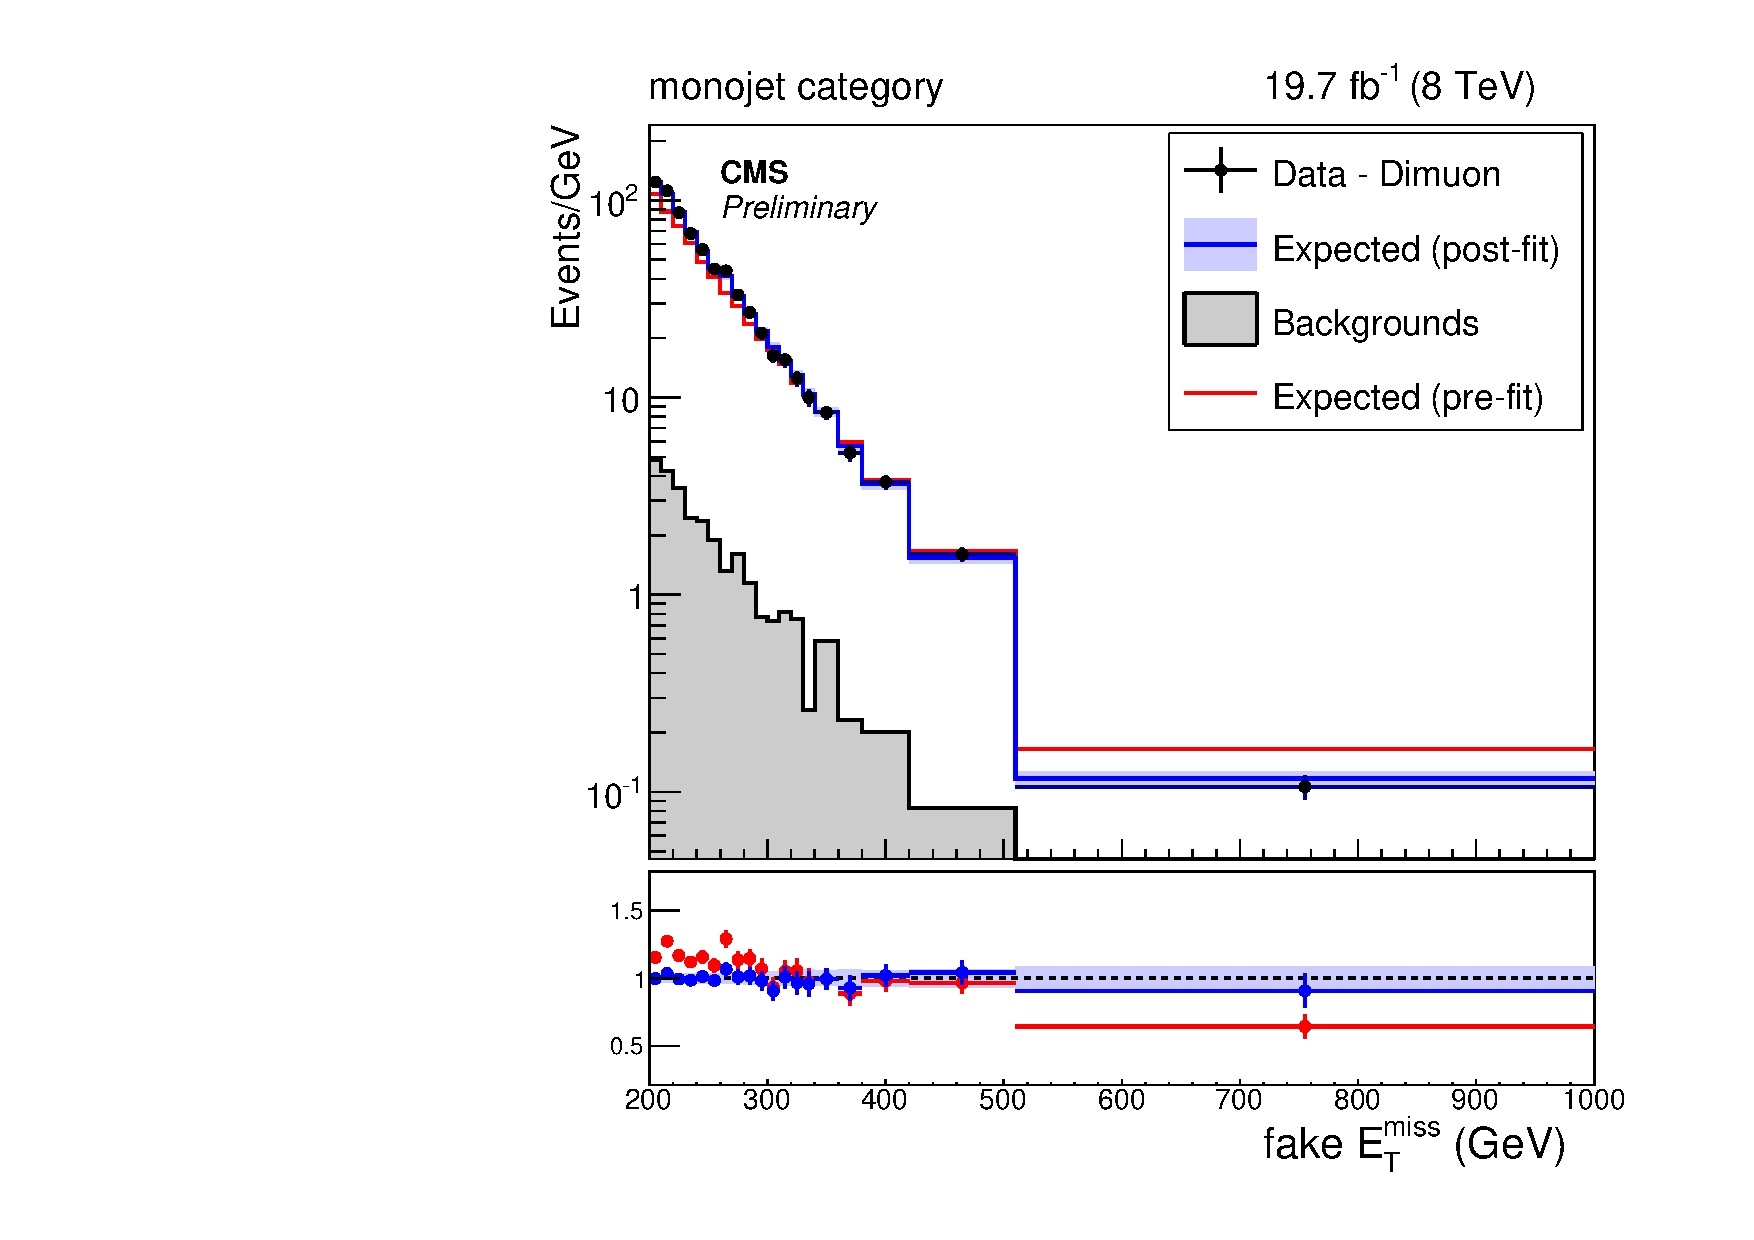
\includegraphics[width=0.32\textwidth]{figures/post_fit_zmm_monojet.pdf}
 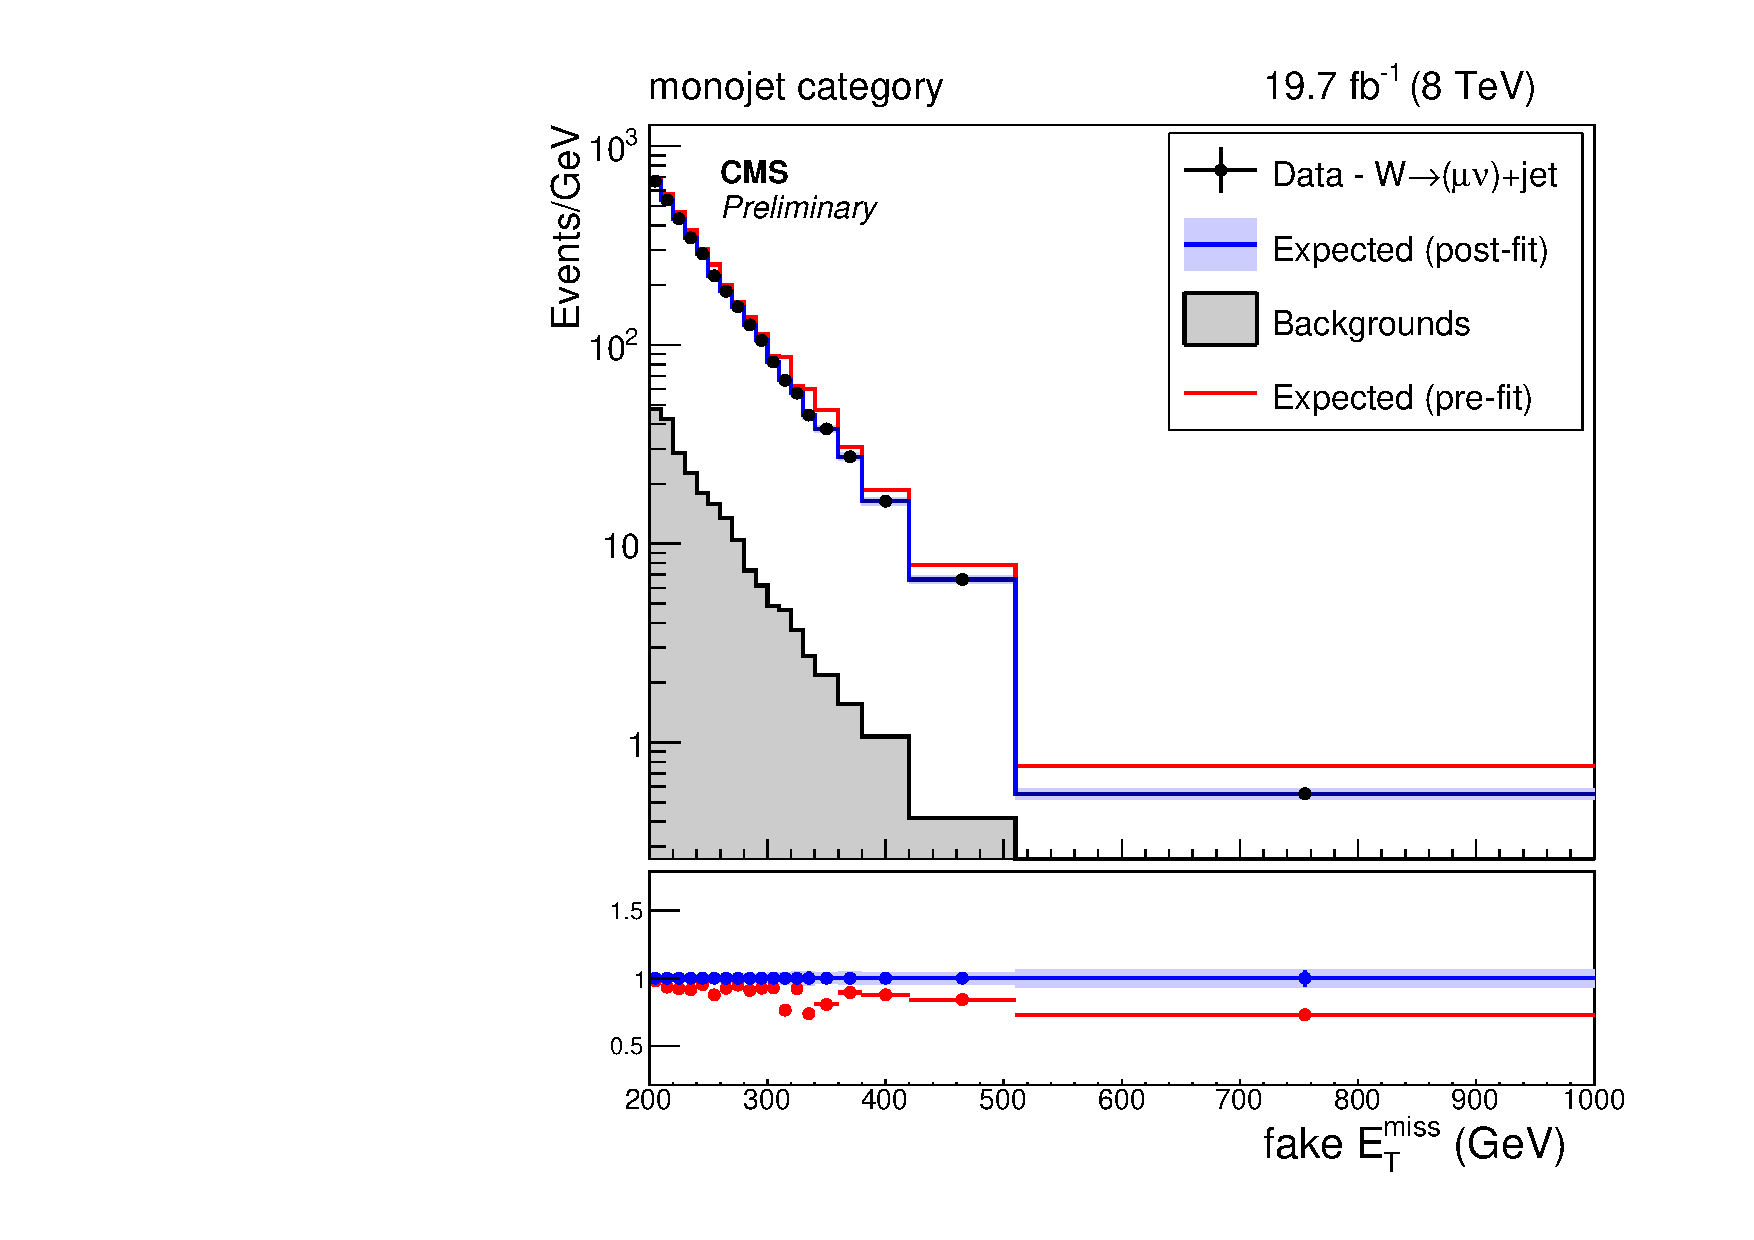
\includegraphics[width=0.32\textwidth]{figures/post_fit_wmn_monojet.pdf}\\
 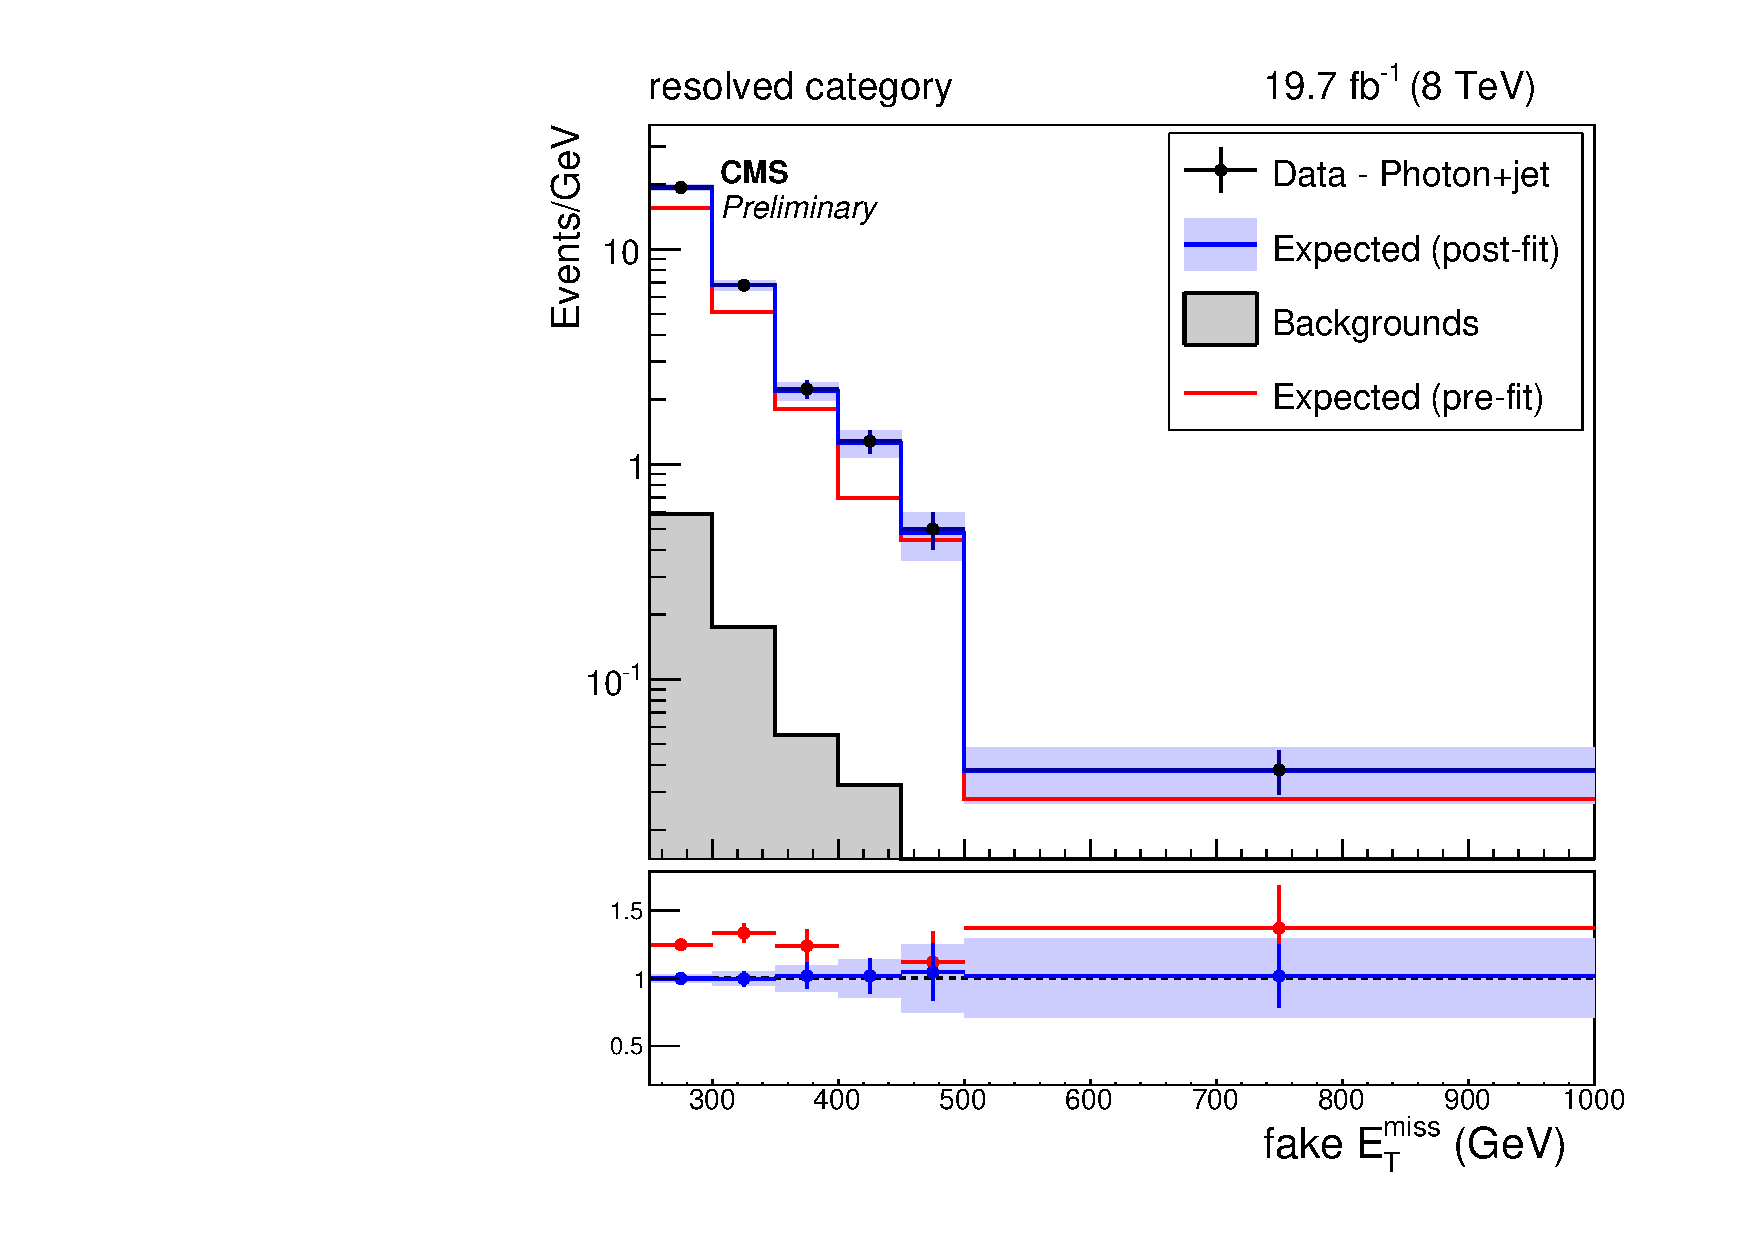
\includegraphics[width=0.32\textwidth]{figures/post_fit_photon_resolved.pdf}
 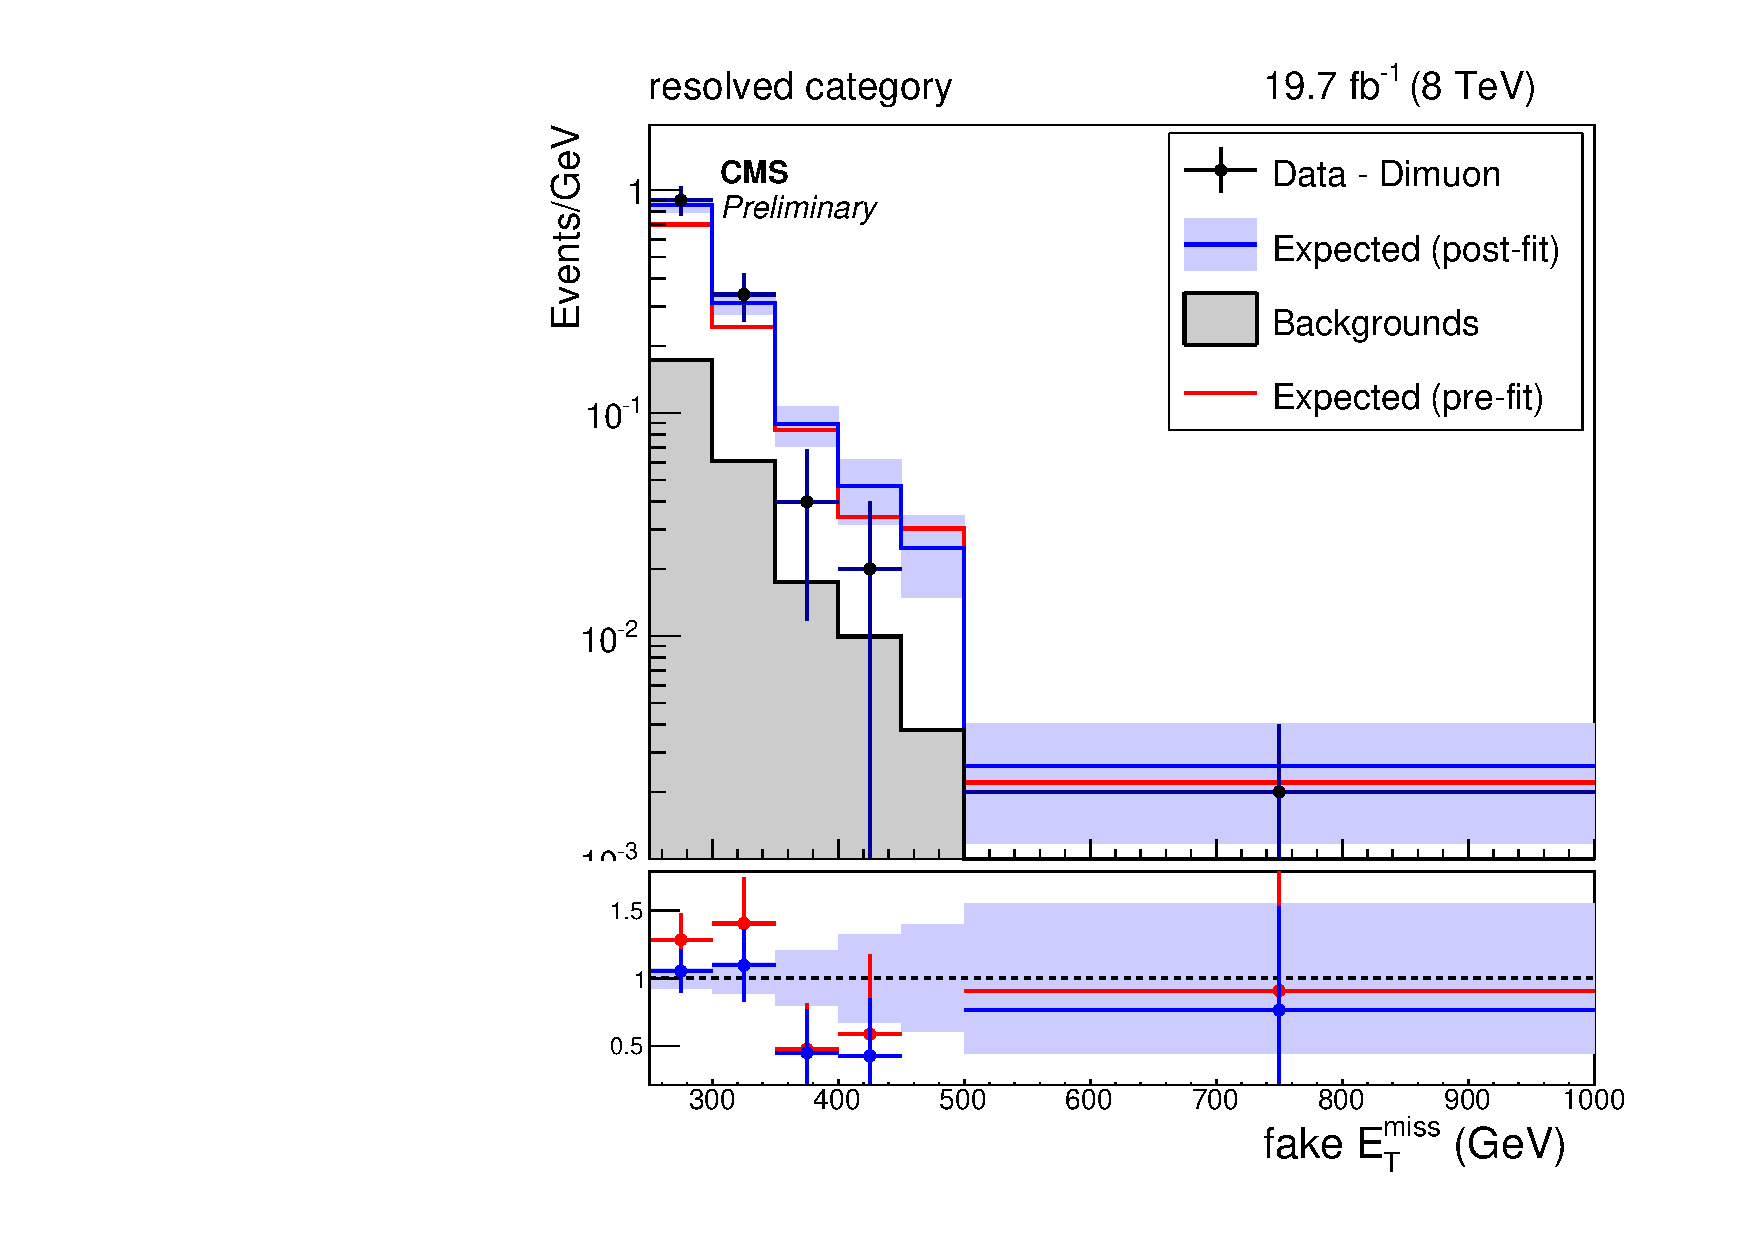
\includegraphics[width=0.32\textwidth]{figures/post_fit_zmm_resolved.pdf}
 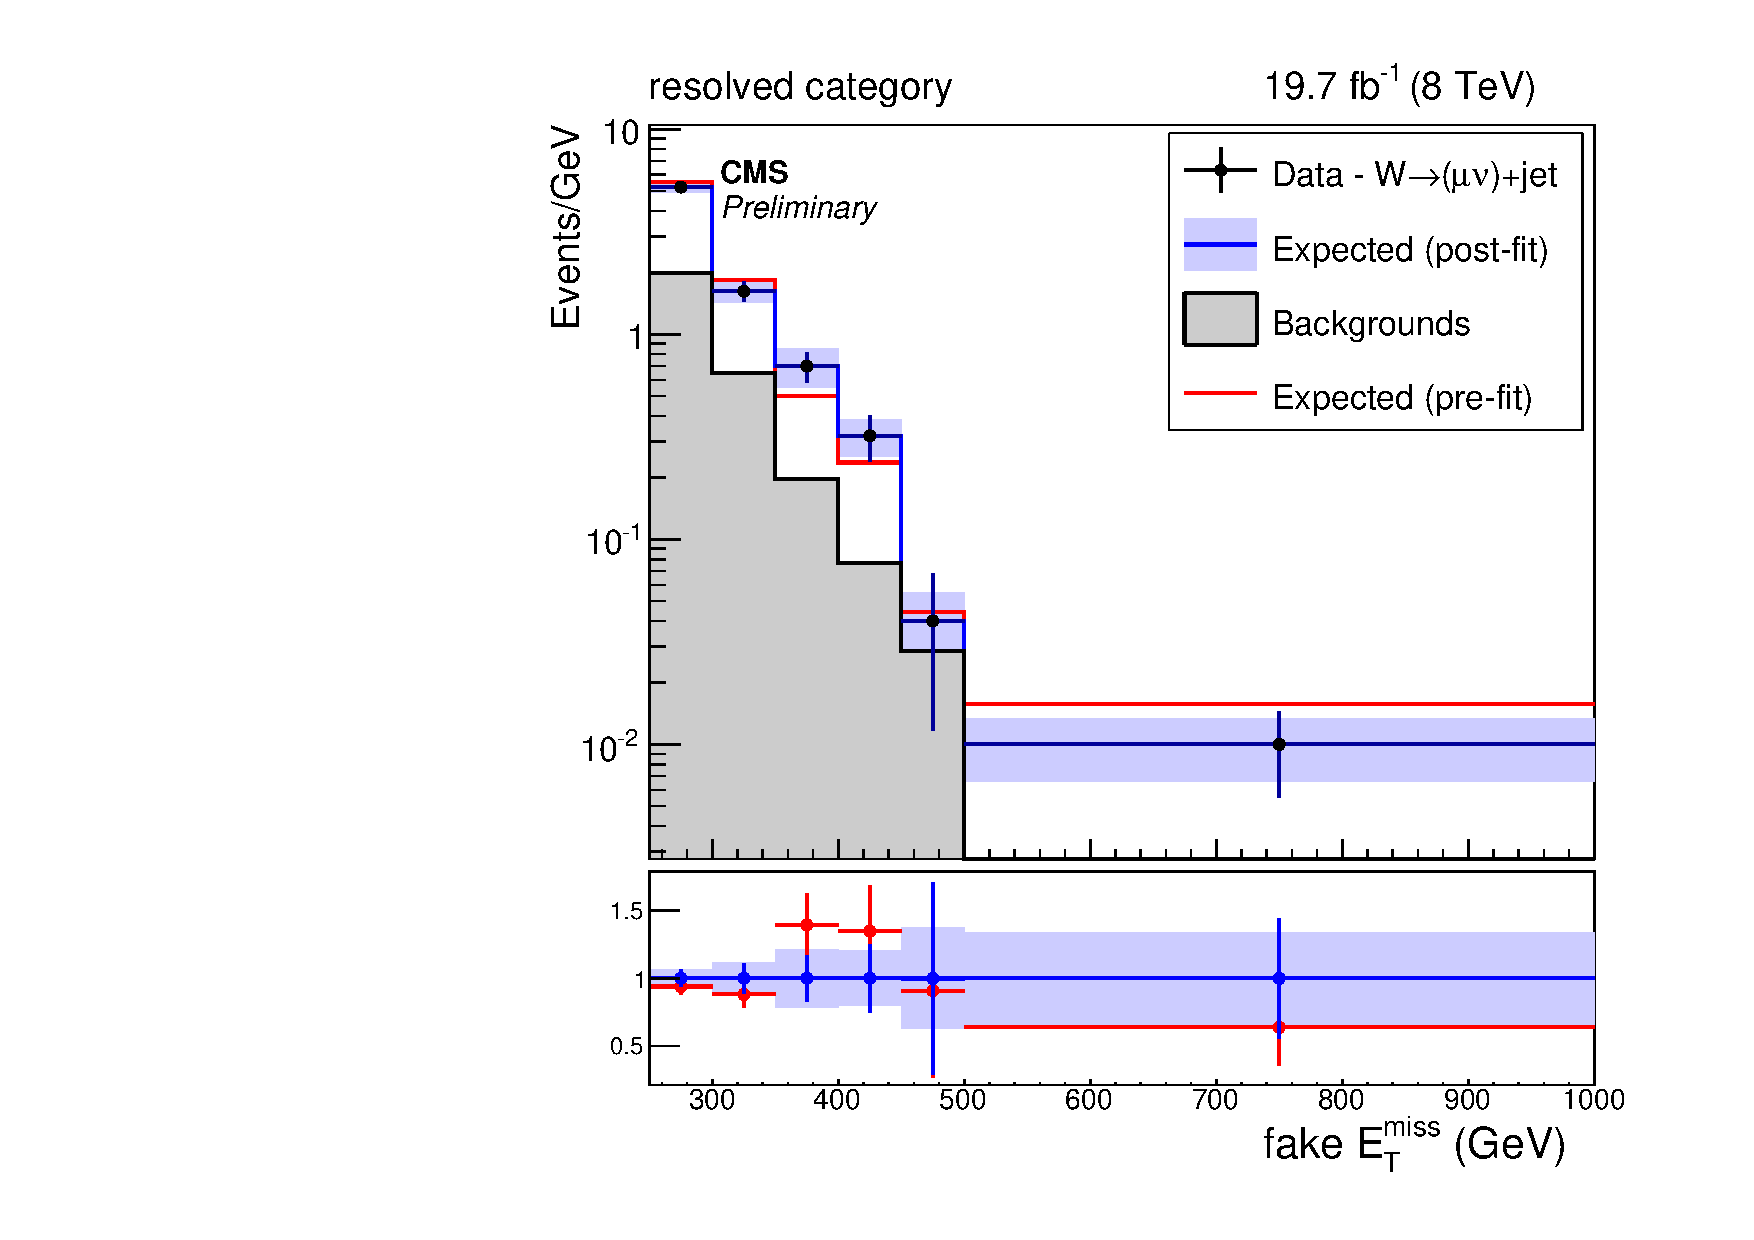
\includegraphics[width=0.32\textwidth]{figures/post_fit_wmn_resolved.pdf}\\
 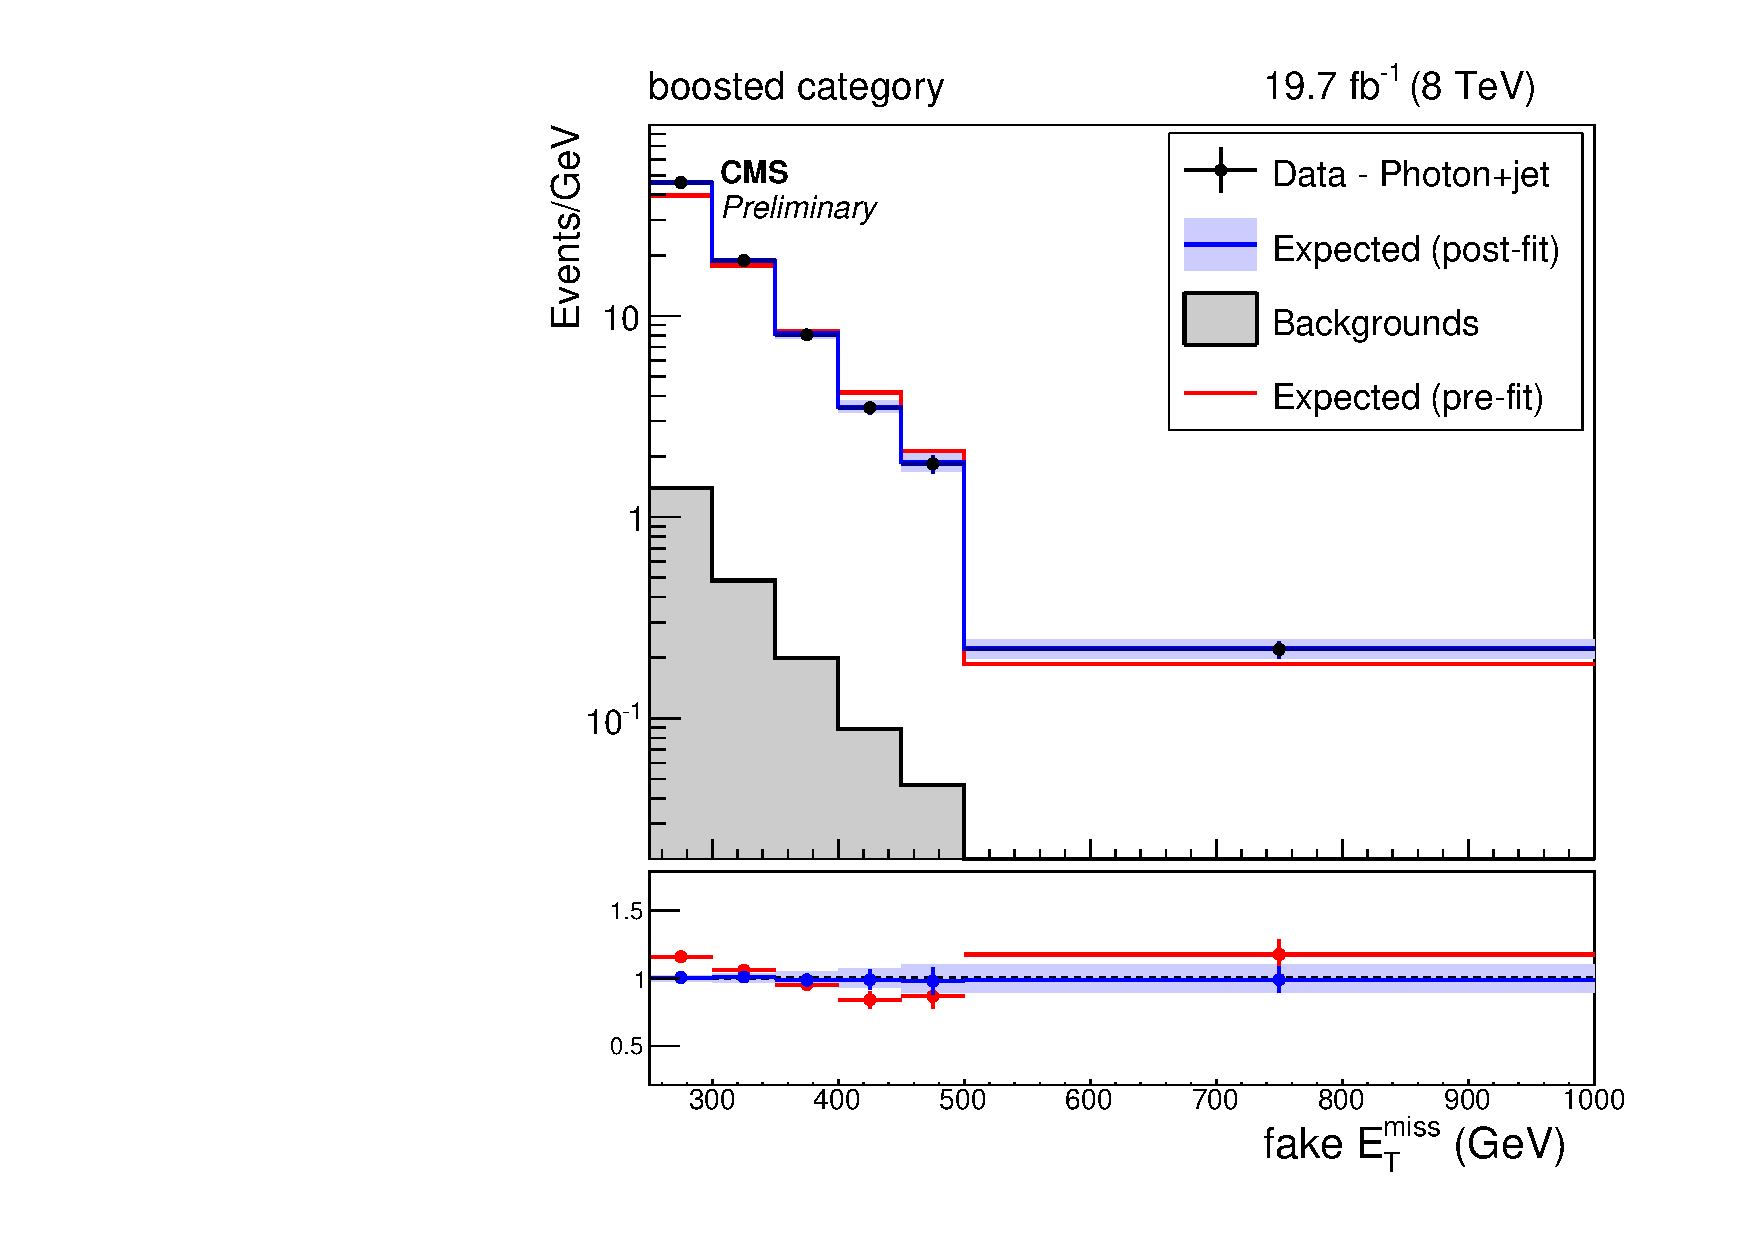
\includegraphics[width=0.32\textwidth]{figures/post_fit_photon_boosted.pdf}
 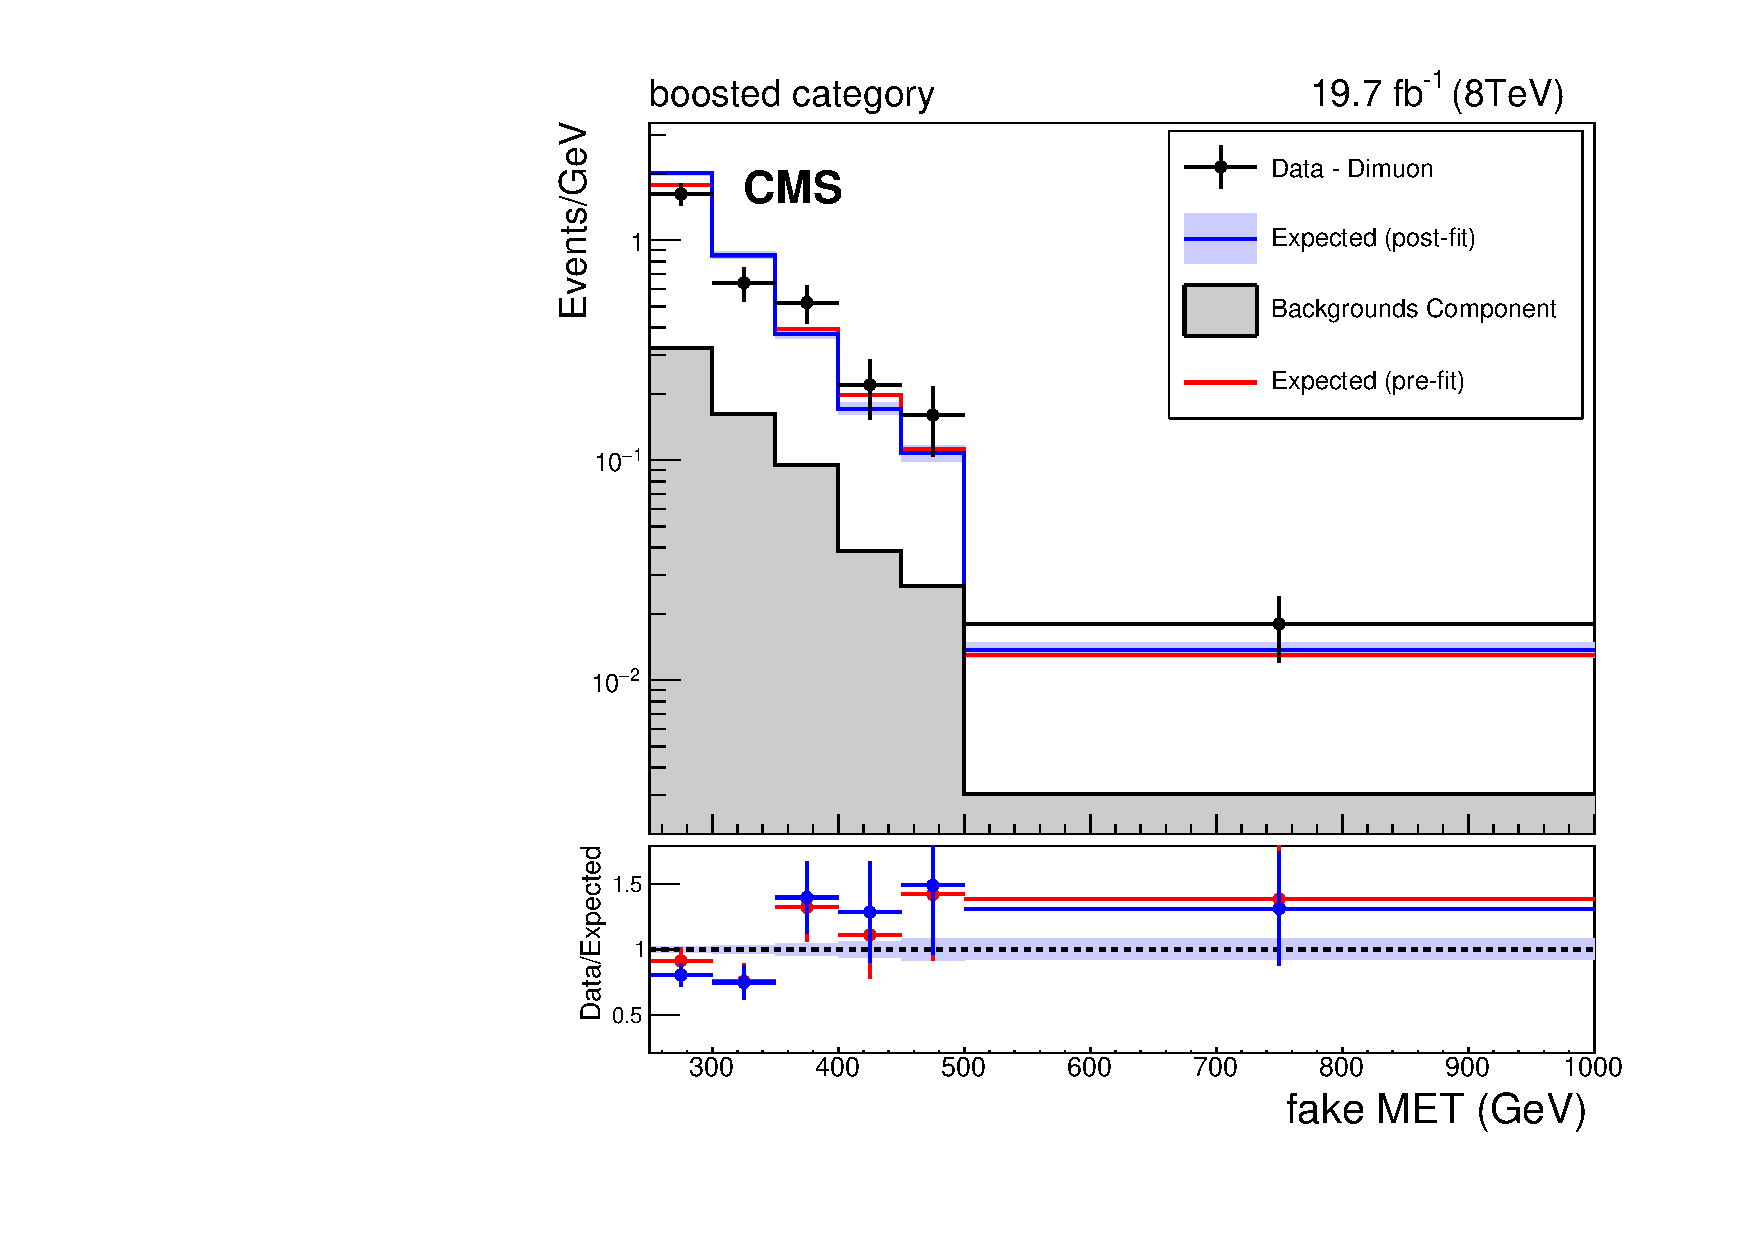
\includegraphics[width=0.32\textwidth]{figures/post_fit_zmm_boosted.pdf}
 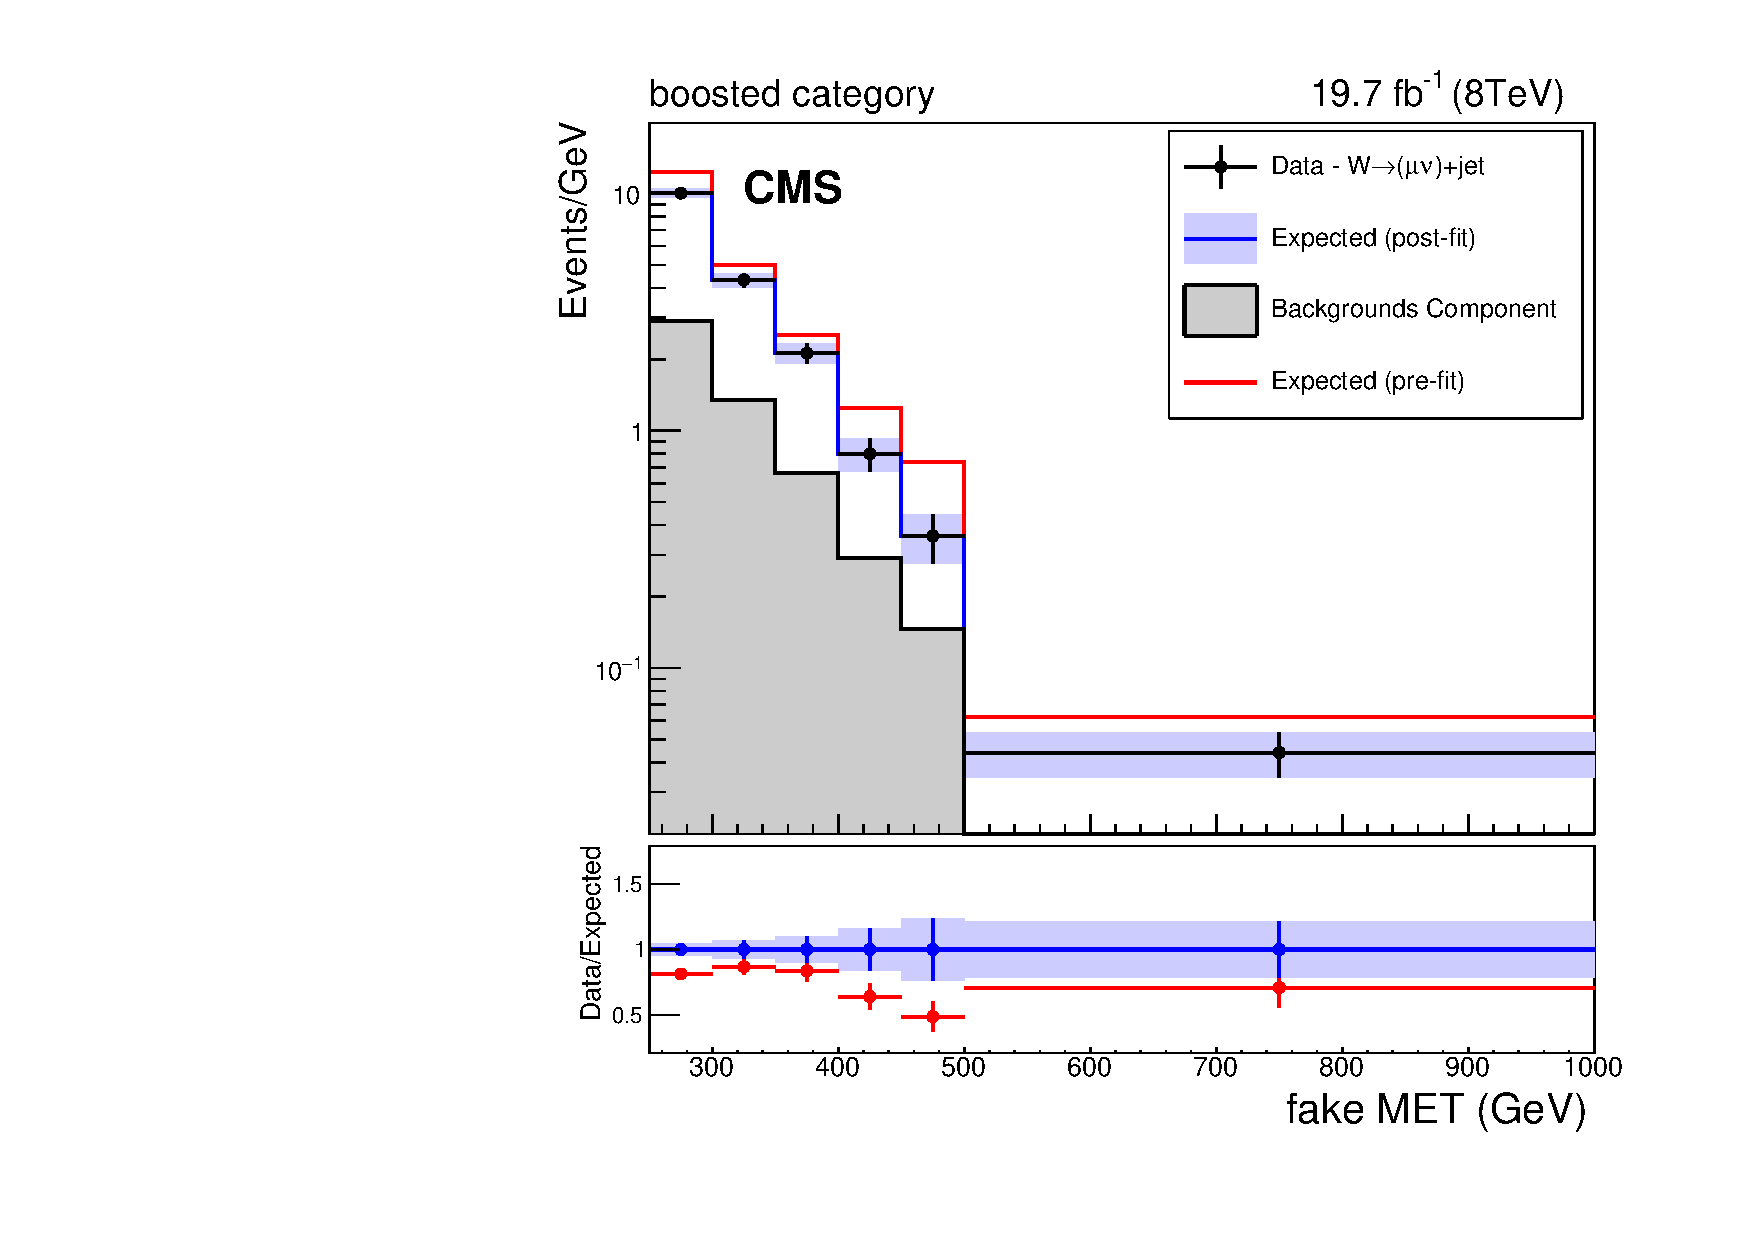
\includegraphics[width=0.32\textwidth]{figures/post_fit_wmn_boosted.pdf}\\
\end{center}
 \caption{Expected and observed fake \ETm distributions in the photon~(\cmsLeft), dimuon (middle) and single-muon~(\cmsRight) 
 control regions after performing the simultaneous likelihood fit to the control regions. 
 Each row, from top to bottom, shows the result of the fit in the monojet, resolved and boosted event categories 
 respectively. The red line represents the expected distribution before fitting to the control regions, while the blue line shows the expectation after 
 the fit. In the ratio, the blue and red points show the ratio of the observed data to the post-fit and pre-fit expectations 
 respectively. The blue bands indicate the statistical and systematic uncertainties from the fit.\label{fig:combined_fit_result} }
\end{figure}

The remaining backgrounds are expected to be much smaller than those from V+jets and are estimated directly from the simulation. 
Shape and normalization systematic uncertainties from the recoil corrections applied to these 
backgrounds are included to account for the uncertainty in the energy scale and resolution 
of jets. Additionally, a systematic uncertainty of 4\% is included for the top backgrounds due to the uncertainty of 
the b-tagging efficiency for the b-jet veto in the resolved category. Systematic uncertainties of 7\%, 10\% and 50\% are included for the top, diboson 
and QCD backgrounds respectively to account for the uncertainty in their production cross-sections. These individual backgrounds have been studied separately using dedicated control regions in data in order to validate these systematic uncertainties. Finally, a systematic uncertainty of 2.6\% in the luminosity 
measurement~\cite{lumi} is included for all of the MC derived backgrounds.


%Table~\ref{tab:systematics} gives a summary of the systematic uncertainties on the backgrounds estimation which are propagated to the calculation of the limits.
%Experimental uncertainties in the signal resulting from jet energy scale and resolution and V-tagging efficiency are included in the signal model for all of the interpretations described.

%\begin{table*}[htbp]
%  \begin{center}
%    \topcaption{Systematic uncertainties and their relative effect on the expectation for the SM backgrounds. 
%      \label{tab:systematics}}
%    %\small
%    \begin{tabular}{llccc}
%      \hline
%      \hline
%      Systematic Uncertainty 	   	            & Process & Boosted & Resolved & Monojet  \\
%      \hline
%      \hline
%      Control region fits$^{\dagger}$ & $\Zvvjets$  &6-20\%  &7.6-44\%  &2.5-9.5\%  \\
%      			   	      & $\Wlvjets$  &10.5-55\% &14.5-320\%  &3.6-17\%  \\
%      \hline
%      Tau-id efficiency		& $\Wlvjets$      & 3.6\% & 3.6\% & 3.6\% \\
%      \hline
%      V-tag efficiency$^{\ddagger}$ 		& Dibosons, Top & \multicolumn{2}{c}{10\%,6\% } &  \\ 
%      \hline
%      b-tag efficiency 		& Top & \multicolumn{3}{c}{4\% } \\ 
%      \hline
%      \ETm recoil 		& Dibosons      & 0.6\% & 2.8\% & 0.3\%  \\ 
%       				& Top    	& 1.1\% & 1.8\% & 1.3\%  \\ 
%       				& $\Zlljets$    & 5.8\% & 9.4\% & 0.7\%  \\ 
%      \hline
%      $t\bar{t}$ norm  		& Top 	      & 7\%  & 7\%  & 7\% \\ 
%      Dibosons norm 		& Dibosons    & 10\% & 10\% & 10\%\\ 
%      QCD norm		 	& QCD 	      & 50\% & 50\% & 50\%\\ 
%      \hline
%      Luminosity  	 	& All except V+jets  & 2.6\% & 2.6\% & 2.6\% \\ 
%      \hline 
%      \hline
%    \end{tabular}\\
%    \end{center}
%    \bottomcaption{\footnotesize{$^{\dagger}$ The relevant components of the fit uncertainties relating to theory and muon/photon identification scale-factors 
%	in the control regions, described in Section~\ref{sec:zjetsmodel}, are included here and correlated between event categories.
%	The numbers here indicate the range of the size of the uncertainties (the smallest to largest) in any \ETm bin due to these fits but should not be 
%	interpreted as the systematic uncertainty which is propagated to the signal extraction.
%	For the boosted category, the uncertainty of 320\% is simply the result of a small fitted yield in one of the bins of the single muon control region.\\
%	$^{\ddagger}$ Uncertainty modeled as migration between the V-tagged (boosted and resolved) and monojet categories.
%    }}
%\end{table*}

